\documentclass[aspectratio=169]{beamer}
%% For 4:3 aspect ratio:
%% \documentclass{beamer}
\usepackage{../git-course}

\title[git-course]{An Introduction to \gh\ and \gs}
\author{Andrew Edwards}
\date{\today}

\begin{document}
%% Needed to remove 'Figure:' from figure captions:
\setbeamertemplate{caption}{\raggedright\insertcaption\par}

\frame[plain]{
\titlepage
}

\section{Definitions}
\frame{\frametitle{Definitions}
  \bi
  \item Repository -- essentially a directory containing all your files for a
    project (plus some files that Git uses).
  \item Git -- a program that allows you to efficiently save ongoing versions of
    your files (`version control').
 \item GitHub -- a website that hosts your repositories so that you can easily
   share code and collaborate with colleagues.
  \ei

Basically, you work on your files in a repository on your computer, use Git on
your computer when you are happy with some changes, and share the files easily on GitHub.
}


\section{Contents}

\frame{\frametitle{Contents}
\bn
\item Creating -- create a new repository on \gh
\item Cloning -- copying it to your local computer
\item Committing -- the crux of working with Git
\item Collaborating -- efficiently work with colleagues
\item Conflicts -- fixing conflict changes (happens rarely)
\item Congratulations -- you now know the basics, summarised on a page
  \en
  \bigskip
We will demonstrate the basics in this video lecture, which includes three
exercises for you (you need a partner for the third one).
}

\section{Creating}
\frame{\frametitle{Creating a new repository}
  \bi
    \item Sign into your \gh\ account, click on the
      \emph{Repositories} tab, and press the \emph{New} button.
    \item Give your repository a name. Let's call it \lst{test}.
    \item Check \emph{Initialize this repository with a README}.
    \item Leave \emph{`Add .gitignore`} and \emph{`Add a license`}
      set to \emph{None}.
    \item Click \emph{Create repository}.
  \ei

You now have a new repository on the \gh\ website. Next we will \lst{clone} it
onto your computer.
}

\section{Cloning}
\frame{\frametitle{Cloning your new repository}
  \bi
    \item Copy the full URL (web address) of your test repository.
    \item Open the \gs\ and navigated to your \lst{C:/github} directory
      (or whatever you called it when you created it in the setup instructions
      -- it's the place you are going to save all your Git repositories).
    \item run the following command to \emph{clone} your repository:

      ~~\lst{git clone URL}\\
      where \lst{URL} is the url of your newly created repository (paste should work).
  \ei
  ~\\
  You should now have a subdirectory called \lst{github/test} on your computer.\\

  In \gs, change
  to that directory:\\
  ~~\lst{cd test}
  ~\\

  So `clone' is Git speak for copying something from GitHub onto your local
  computer.
  ~\\
  This example has just one file (the README). But the process is the same for a
  repository with multiple files and multiple directories (the structure is
  fully preserved).
}

\frame{\frametitle{Windows only: Storing your credentials}
  When you are using the \gs\ for the \alert{very first time on Windows}, issue
  the following command:\\
  \bigskip
  \lst{git config --global credential.helper wincred}\\
  \bigskip
  This means that you don't have to repeatedly enter your \gh\ password (just do
  it when you are first prompted).\\
}

\section{Committing}
\begingroup
\small
\frame{\frametitle{Creating and committing a new file}
  \bi
    \item Create a new file, \emph{newFile.txt}, in the \lst{github/test}
      directory.
    \pause
    \item Add a line of text at the start of the file and save it.
    \pause
  \item Check the status of the (\lst{test}) repository by typing
    \lst{git status} in the Git shell.
    \pause
  \item It should say that you have an `Untracked file' called \emph{newFile.txt}.
      You want to tell Git to start tracking it, by using the \lst{git add}
      command:\\
      \lst{git add newFile.txt}
   \pause
 \item Type \lst{git status} again. (If on MacOS you may see mention of a
   \emph{.DS\_Store} file -- ignore that for now).
 \item You should see that the file is listed as a `new file` under `Changes to
   be committed`.
    \item Let's now `commit' it:\\
      \lst{git commit -a -m "Add newFile.txt file."}\\
      The commit message should be a useful message saying what the commit
      encapsulates.\\
    \pause
    \item Push the commit to \gh: \lst{git push}
    \pause
    \item Check (refresh) the \gh\ webpage and see your commit and the uploaded file.
  \ei
}
\endgroup

\frame{\frametitle{What just happened?}
  We just used three of the main Git commands:
  \bi
  \item \lst{git add <filename>} -- tell Git to start keeping track of changes
    to this file. You only need to tell Git this once.
  \item \lst{git commit -a -m "Message."} -- committing your changes, which means tell Git
    you are happy with your edits and want to save them. % You are actually saving
    % a snapshot of your entire repository (all the folders and files in your repository).
  \item \lst{git push} -- this sends your commit to the GitHub website.
  \ei

 You always have your files stored \emph{locally} on your computer (as usual),
 even if you don't \lst{add} them or \lst{commit} changes.

 ~\\

 When you push to GitHub then your colleagues can easily \lst{fetch} (retrieve) them.
}

\frame{\frametitle{Keyboard aliases (shortcuts)}
Now, \lst{git commit -a -m "Message."} is a bit much to type, so we have an
alias for it:

~\\

\lst{git com "Message."}

~\\

This is defined in the \emph{.gitconfig} file you installed in the `git-setup`
instructions.

~\\

The \lst{-a} means `commit all changes of files that Git is tracking`, and \lst{-m} is
to include a message. Since we usually want to do both of
these, \lst{git com "Message."} is a useful shortcut. But it is important to
realise it is an alias if searching online for help.

Similarly:

\lst{git s} -- for \lst{git status}

\lst{git p} -- for \lst{git push}

\lst{git d} -- for \lst{git diff}

From now on we will use the aliases.
}

\frame{\frametitle{Edit \emph{Readme.md}}
  Edit the \emph{Readme.md} file. Add some simple comments describing
  the project such as: ``A test repository for learning Git.''\\
  \bigskip
  \pause
  Look over the changes, commit them, and push them to your \gh\
  repository:\\
  \lst{git s}\\
  \lst{git diff} or the alias \lst{git d} -- this gives a simple look at the differences between the last committed
  version and your current version (of all files; only one in this case) \\
  \lst{git com "Initial edit of Readme.md"}\\
  \lst{git p}\\
  ~\\
  Refresh your \gh\ web page and you should see your text
  (the \emph{Readme.md} file is what is shown on the main page
  of your repo).
}

\frame{\frametitle{Exercise 1: create, edit, and commit \emph{simpleText.txt}}
  \bn
    \item Create a text file \lst{simpleText.txt}
      in your local \lst{test} repository. Add a line of text at the start and
      save it.
    \pause
    \item Predict what \lst{git s} will tell you, \emph{then} type it in the
      Git shell to check.\\
    \pause
    \item Add the file to the repository using the git commands:\\
      \lst{git add simpleText.txt}\\
      \lst{git s} -- not necessary but useful to check you understand what is
      changing before you commit\\
      \lst{git com "Adding simpleText.txt"}\\
      \lst{git p}
    \pause
    \item Add some text to \lst{simpleText.txt}, then \lst{git com "Message"} and \lst{git p}.
    \pause
    \item Repeat this a few times to get the hang of it, while intermittently doing \lst{git s} and
      \lst{git d} to understand what's changing.
    \pause
    \item Keep an eye on your commits by refreshing the \gh\ page.
  \en
}

\frame{\frametitle{Adding multiple files at once -- slide 1}
  Often you add multiple files in a new directory. When you run \lst{git s}, you
  will see a large list of \emph{Untracked files}. They can be added at once by simply
  adding the whole directory.
  \bi
    \item Create a new directory to your \lst{test} repository, using your normal method. Call it \lst{new-stuff}.
    \item Add a few new test files to that directory called
      \lst{test1.txt}, \lst{test2.txt}, etc. Put some example text
      in one or more of them if you want.
    \item On the command line, check the status:\\
      \lst{git s}
    \item You will see a listing showing the \lst{new-stuff} directory in
      \emph{Untracked files}.
%    \item To see the actual files to be committed instead of just the
%      directory:\\
%      \lst{git s -u}
    \item To add all the new files in preparation for a commit,
      issue the command:\\
      \lst{git add new-stuff/}
  \ei
  \bigskip
  Continued...
}

\frame{\frametitle{Adding multiple files at once -- slide 2}
  \bi
    \item Check the status of the repository again:
      \lst{git s}
    \item It will now show all files in \emph{Changes to be committed}
    \item Commit the changes:\\
      \lst{git com "Added new-stuff directory."}
    \item Push the changes to \gh:\\
      \lst{git p}
    \item Check your \gh\ webpage and see your commit and that the files
      have been uploaded.
    \item That works no matter how many files are in your \lst{new-stuff}
      directory.
      \ei
  Exercise 2: Try the above, to practice creating multiple files in a folder and
  committing that folder.
}

\frame{\frametitle{Adding multiple files at once -- slide 3}
  \bi
    \item To add multiple files with similar names you can use the wildcard
      \lst{*} symbol.
    \item You just added (told Git to keep track of) the new files in your
      \lst{new-stuff/} directory.
    \item If you add more new files to that directory, you will
      have to tell Git to track those also (since they are new -- you haven't
      told Git about them yet).
    \item Say you have 10 new files in \lst{new-stuff/} called \lst{idea1.txt}, \lst{idea2.txt}, ..., \lst{idea10.txt}.
    \item Instead of typing\\
      \lst{git add new-stuff/idea1.txt}\\
      \lst{git add new-stuff/idea2.txt}\\
      etc. (note the \lst{new-stuff/} folder name there)
      you can just use the wildcard \lst{*}:\\
      \lst{git add new-stuff/idea*.txt}\\
      (or even just \lst{git add new-stuff/*.txt}, or \lst{git add new-stuff/*.*}).
    \item No need to do this now, but this is useful to know.
  \ei
}


\frame{\frametitle{The \emph{.gitignore} file}
  But what if you don't want to add all the files that you create?

  ~\\

  Each repository can have a \emph{.gitignore} file, in the root directory
  of the repository.

  Such a file has names of files (such as \lst{my-secret-notes.txt}) or wildcard names (such as
  \lst{*.pdf} or \lst{*.doc}) that will be completely ignored by Git.

  ~\\

  When sharing a repository with others, you want to share your \emph{code} (for
  example, R or Python code) and maybe data, but generally \emph{not} share the output (such as figures
  that the code generates; more on this later). For reproducible research your colleague (or anyone)
  should be able to run your code to generate the results.

  ~\\

  Some programs you run may make temporary files that don't need to be tracked
  by Git, the names of which should also be included in your \emph{.gitignore}.
}

\frame{\frametitle{The \emph{.gitignore} file}
  When sharing code or collaborating you want to keep your
  repository as clean as possible and not clutter it up with files that other
  people don't need.

  ~\\

  So when you run \lst{git s} and see untracked files that you don't want to be
  tracked, add them (or a suitable wildcard expression) to your
  \emph{.gitignore} file so that they are not added inadvertently.

  ~\\

  This will also simplify your workflow (you don't need to keep being reminded
  that you have untracked files).

  ~\\
  If you are on MacOS and you find that folders have a \emph{.DS\_Store} file
  in them, then create (and add and commit) a \emph{.gitignore} file with \emph{.DS\_Store} as a line.
}

\frame{\frametitle{Thoughts/hints regarding commit messages}
  What to write in \lst{git com "Message"}?\\
  Ideally:
  \bi
    \item Want to describe \emph{what} and (sometimes \emph{why}) you did
       something.
    \item The \emph{how} is not needed since that will be explained by the
       actual changes in the code.
    \item Message should be informative for collaborators (including your future self).
  \ei
  {\red Bad}:\\
  ~~\lst{git com "Tweaked function."}\\
  {\blue Good}:\\
  ~~\lst{git com "Allow plot.biomass() to use extra colours."}\\
}


\section{Collaborating}
\frame{\frametitle{Git Workflow}
  You have now learnt the basics of using Git. By creating a public repository
  on \gh\ you can now release your code to the world!

  ~\\
  You can also choose the \emph{private repository} option when creating a
  repository, so that you can control who can see it.

  ~\\

  Now we will show how to collaborate with colleagues, which is where the
  usefulness of Git will become more apparent.
}


\frame{\frametitle{Git Workflow}
  There are a few different ways to collaborate using Git and \gh. We will focus on the
  following one since it is the simplest, and is what you need to collaborate
  with colleagues.

  ~\\

 Concept: there is a project where people contribute to a main repository that is
      considered the `master copy'.
      \bi
        \item Everyone clones directly from the creator's repository.
        \item All collaborators push their commits to the main
          repository (the creator has to
          grant them permission once on \gh).
      \ei

Since the creator has to grant permission, you won't have just anyone
contributing to (and maybe messing up your work), just your team.

~\\
But you have to trust your team to not mess things up (more on that later).

}


\frame{\frametitle{Demonstration of collaborating}
  \bi
    \item Kim creates new repo called \lst{collaborate} (and clones it to her computer).
    \item Andy clones it also.
    \item On \gh, Kim gives Andy `push access' to her \lst{collaborate} repo.
    \item Both do some edits (create some new simple text files).
    %  keeping an eye on the evolving Network Graphs.
    \item For Andy to get Kim's updates (and vice versa), it will just be:
    \bi
      \item \lst{git fetch} -- this fetches the latest version of the repository from
        \gh\ onto your computer. Your local files have \emph{not} yet changed
        (check them),
        but Git has the changes stored on your computer (!).
      \item \lst{git rebase}  -- this updates your local
        repository (the committed files on your computer) with the changes you
        have just fetched, merging both people's work together.
      \item \lst{git p} -- this pushes the merged changes back up to \gh\ so
        that the other person can get them.
    \ei
  \ei
}

\frame{\frametitle{Demonstration of collaborating}
We will show an example of \lst{git p} \emph{not} being allowed
  because there are changes on \gh\ (by someone else) that you have not yet merged into your local
  repository.

  ~\\

  You need to deal with these first by \lst{git f} and then \lst{git
    rebase}. Here is an example of the error message you get:\\

  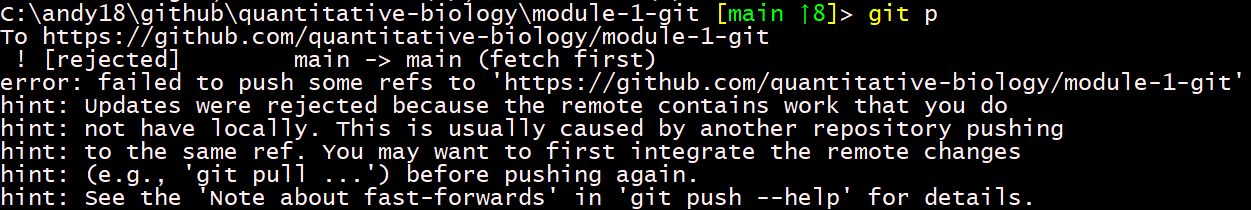
\includegraphics[
  width=0.8\textwidth,
  keepaspectratio]{figures/unable-to-pull}

  While a bit lengthy, the error message is useful. It forces you to get the
  other person's work before you push yours.
}

\frame{\frametitle{Demonstration of collaborating}
  So to be allowed to push, just fetch and then rebase (which combines the commits):
  \bi
\item \lst{git f}
\item \lst{git rebase}
\item \lst{git push}
  \ei
  See next page for a full screenshot.
}

\frame{\frametitle{Demonstration of collaborating}
Here is a full screenshot (`g` is just a shortcut for `git`). The green uparrow
number 8 tells me I have 8 commits to push to \gh. The yellow arrows I think of
as just implying I need to do a rebase:

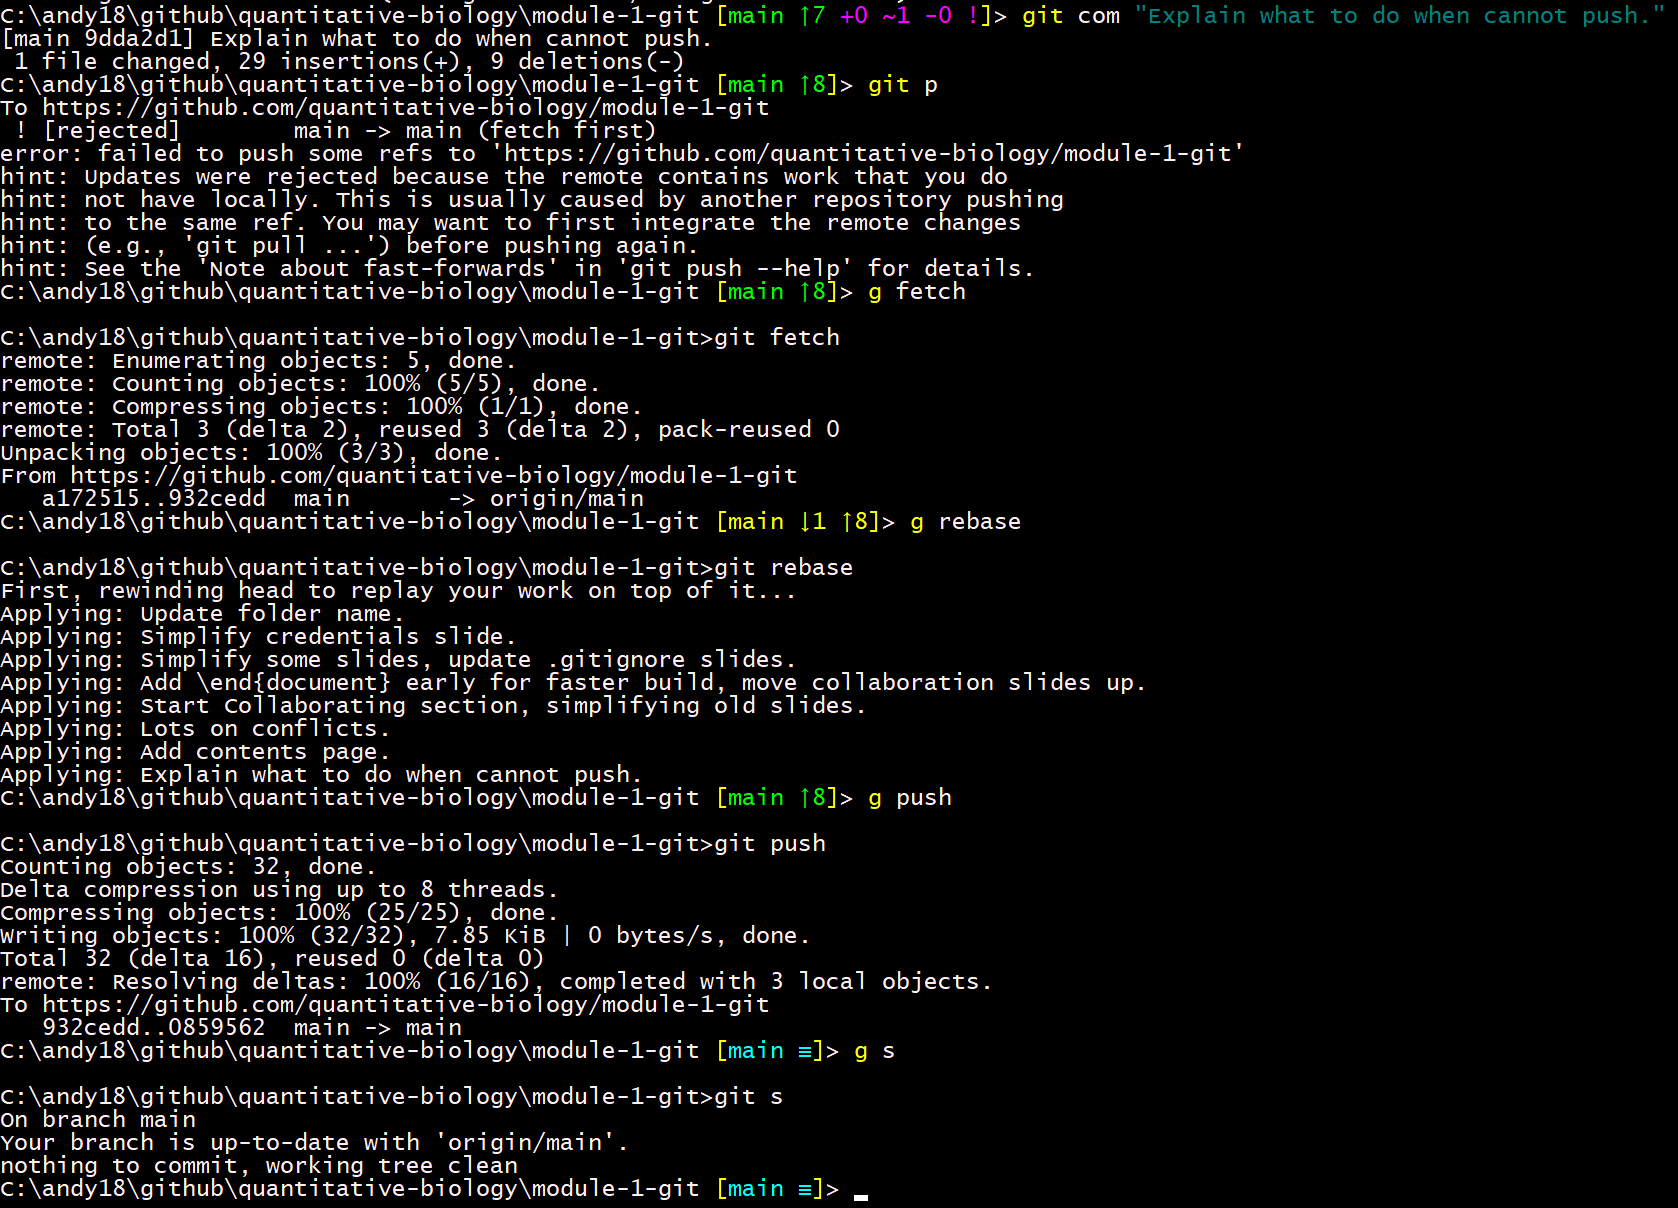
\includegraphics[
  width=0.55\textwidth,
  keepaspectratio]{figures/fix-the-pull}
}





\frame{\frametitle{A bit more about \lst{git rebase}}
\bi
  \item Andy commits local changes, tries to \lst{git push} but is told to first
    \lst{git fetch} (to get Kim's changes from \gh).
  \item Andy does \lst{git fetch} and then \lst{git rebase}.
  \item What \lst{git rebase} does is basically add Andy's commits to Kim's
    commits (TODO: check it's not the other way around!).
  \item Andy then does \lst{git push} to push his commits to \gh\ (from where
    Kim will \lst{fetch} them when she's ready).
  \item Providing there are no conflicts, this will work fine.
\ei

Another option is to do a \lst{git merge}, which basically creates a new commit
that merges both people's work together.

Our groups used to use \lst{git merge} and now use \lst{git rebase}; some people
don't like \lst{git merge} because it adds extra commits.

For a more in-depth understanding see
https://reflectoring.io/git-rebase-merge/ for one of the
clearer explanations out there concerning \lst{rebase} v \lst{merge}.
}

\section{Conflicts}
\frame{\frametitle{Fixing a conflict}
  \bi
    \item A {\red conflict} happens when two people have edited {\red the same line(s)
      of the same file}.
  \item Conflicts happen relatively rarely and can be generally avoided by
    co-ordinating with collaborators so that you are working on different
    files. But, they will happen and you need to know how to resolve them.
  \item Git \emph{forces} you to explicitly decide whose changes to keep -- this
    is a {\red good} thing, since you want a human to make such a decision.
  \ei

We will demonstrate a conflict.
}

\frame{\frametitle{Fixing a conflict}
The best approach I have found to fixing a conflict is the following:
  \bi
\item Trying \lst{git rebase} will tell you there is a conflict.
\item \lst{git rebase --abort} -- do this to abort the rebase attempt.
\item \lst{git merge} -- this will tell you there is a conflict.
\item Open the file(s) with the conflict and edit the text (next slide).
\item \lst{git add <filename(s)>} -- you have to then add the files that had the
  conflict (I am not sure why this is necessary, I just do it).
\item \lst{git com "<message>"} -- in your commit message you can explain how
  you fixed the conflict. This is useful so that your collaborators know you have
  resolved a conflict (they can look at the commit to see if they are happy with
  it).
\ei
}

\begingroup
\small
\frame{\frametitle{Fixing a conflict}
  The merge message will tell you which files are conflicting. Open those
  files one by one, and you will see the conflicted section bracketed like the
  following:\\
  \bigskip
  \lst{<<<<<<< HEAD}\\
  ~~Line(s) of text/code which are currently in your file.\\
  \lst{=======}\\
  ~~Line(s) of text/code which are trying to merge in, but conflict.\\
  \lst{>>>>>>> origin/main}\\
  \bigskip
  where \lst{origin/main} refers to the version you have fetched from \gh.
  ~\\

  All you do is remove the line(s) of text that you do not want to keep (or edit
  the line(s) to be something else entirely), and remove the
  bracketing lines \lst{<<<...} and \lst{>>>...}, and
  the \lst{=======} line.

  Save each conflicted file and then (as mentioned previously):\\
  \lst{git add <filename(s)>}\\
  \lst{git com "Kept Kim's edits as more consistent with
  remaining text."}\\
  \lst{git p}
}
\endgroup


\frame{\frametitle{Exercise 3: collaborating on a single repository}
  If you have a colleague available, try what we just did:
  \bi
\item Person 1 creates a new repository on \gh\ and clone to their computer.
\item Give the Person 2 `push access' to the repository (on the repo page on
  \gh: Settings -- Manage access -- Invite a collaborator)
\item Person 2 clones to their computer.
\item Both create a simple text file (use different filenames), add some text
  and, as usual, \lst{add}, \lst{commit}, and \lst{push} it.
\item \lst{git fetch} and \lst{git rebase} to get the other person's file.
\item Continue editing either file, committing, and pushing.
\item If you get the \lst{push} error (shown earlier), refresh the \gh\ repository site to
  see recent commits (click on the XX commits link). You can easily
  spot the other person's recent commits. Click on one (the bold message) to see
  details.
\item Purposefully create a conflict (both edit the same line of the same
  file). Resolve it as described earlier.
\item In practice you won't commit so frequently, this is good to get the hang of it.
  \ei
}

\section{Congratulations}
\frame{\frametitle{Congratulations}
  Congratulations, you now know the few basic commands and functionality needed
  to collaborate with Git and \gh.
  It takes a bit of practice, but it is very powerful.\\

  {\red 95\% of the time, this is all you are doing:}\\
  \bigskip
  Change some code.\\
  \lst{git com "My commit message"}\\
  \lst{git p}\\
  If \gh\ does not allow you to push:\\
  \lst{git fetch}\\
  \lst{git rebase}\\
  If conflicts, then \lst{git rebase --abort}, \lst{git merge}, fix conflicts and:\\
  \lst{git add CONFLICTED_FILE}\\
  \lst{git com "Message"}
  \lst{git p}\\
  \bigskip
  Change some code... repeat...
}

% Andy ending it here, as the rest won't be a recorded lecture. Have moved
% remaining slides into module-1-git-advanced.Rmd and will just edit/remove them
% there.
\end{document}
